\documentclass[12pt]{article}

\usepackage[utf8]{inputenc}
\usepackage[margin=1in]{geometry}
\usepackage{graphicx}
\usepackage{amsmath}
\usepackage{hyperref}

\usepackage{caption}
\usepackage{subcaption}
\usepackage{soul}

\usepackage{fancyhdr}

\pagestyle{fancy}
\fancyhf{}
\lhead{Reading Club, IITB Astro}
\rhead{Celestial Mechanics}
\rfoot{\thepage}

\hypersetup{
	colorlinks=true,
	linkcolor=blue,
	filecolor=magenta,      
	urlcolor=blue,
}

\newtheorem{theorem}{Definition}
\newcommand{\e}{\ensuremath{e}}
\begin{document}
%	\title{Primer on Ellipses}
%	\author{Vedant Shenoy}
%	\date{}
%	\maketitle
	\section{Definition of an ellipse}
	\lfoot{Vedant Prakash Shenoy (December 2019)}
	\begin{theorem}
		An ellipse is the locus of points for which the sum of distances from two fixed points (called \emph{focii}) are equal
	\end{theorem}
	We may also define ellipses as a section of a cone (more precisely, a double cone). This definition provides a connect between ellipses and other conic sections. (Fig. \ref{all_conics}) \\
	A third definition is interesting as it defines all conic sections based on a single parameter: called eccentricity(\e)
	\begin{theorem}
		\label{def_conic}
		A conic section is the locus of all points for which the ratio of distance from a fixed point \emph{(focus)} and perpendicular distance to a fixed line \emph{(directrix)} is a constant, which is known as the eccentricity \e\ of the conic section. From Fig. \ref{def_conic}, we can write
		\begin{equation}
			\rm \frac{FP}{PM} = \e
		\end{equation}
		If {\rm0$<$\e$<$1}, then the conic section is called an \emph{ellipse}.
	\end{theorem}
		\begin{figure}[!h]
		\centering
		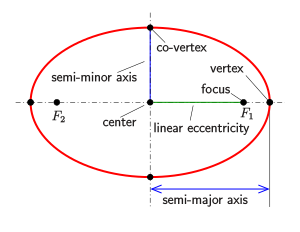
\includegraphics{ellipse.png}
		\caption{Ellipse (Source: \href{https://www.ck12.org/book/CK-12-Algebra-II-with-Trigonometry-Concepts/section/10.0/}{ck12.org})}
		\label{ellipse}
	\end{figure}
	\begin{figure}[!h]
		\centering
		\begin{subfigure}[b]{0.45\textwidth}
			\centering
			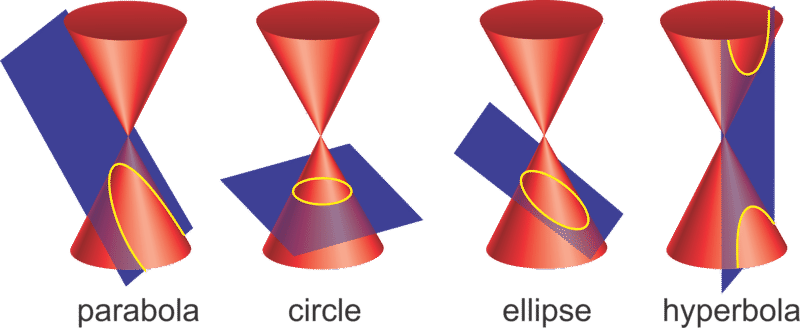
\includegraphics[width=\textwidth]{all_conics.png}
			\caption{Definition of conic sections (Source:~\href{https://upload.wikimedia.org/wikipedia/commons/thumb/9/96/Ellipse-def0.svg/300px-Ellipse-def0.svg.png}{Wikimedia Commons})}
			\label{all_conics}
		\end{subfigure}
		\hfill
		\begin{subfigure}[b]{0.45\textwidth}
			\centering
			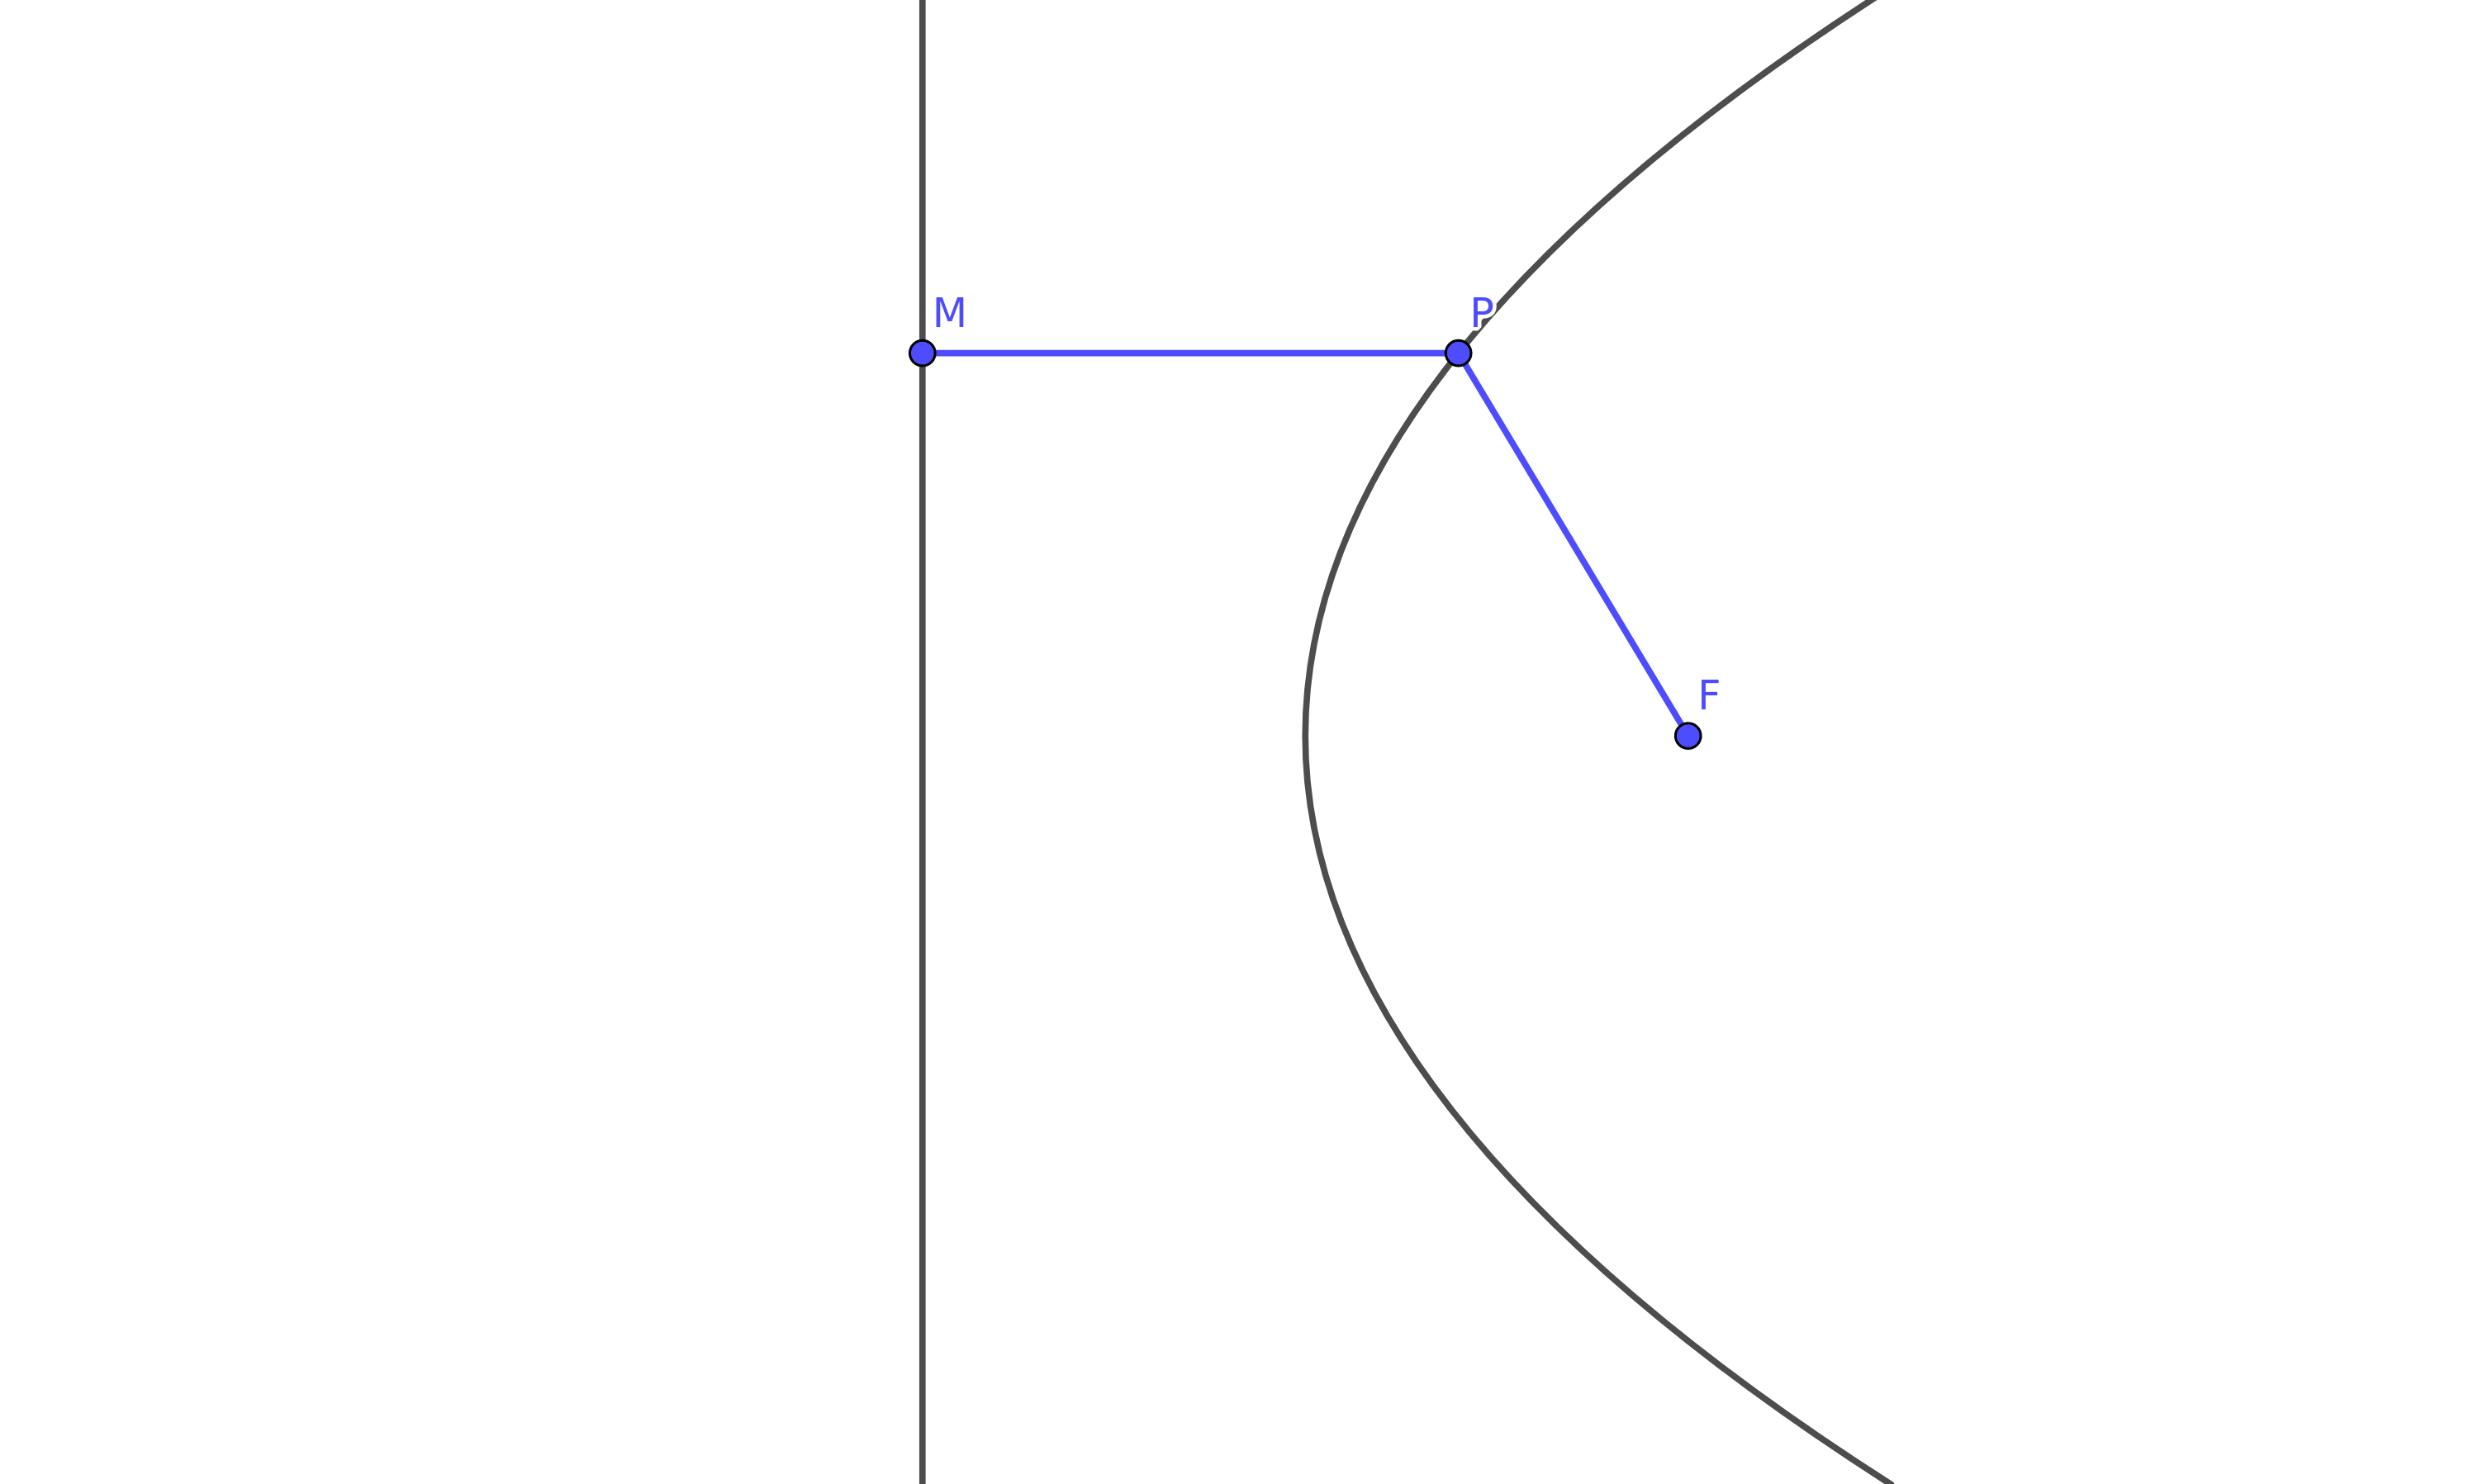
\includegraphics[width=\textwidth]{conic.png}
			\caption{Definition 2. of a conic (Source:~Adapted from Fig 11.6 of \href{http://ncert.nic.in/ncerts/l/keep211.pdf}{NCERT Class 11}}
			\label{def_conic}
		\end{subfigure}
		\hfill
		\caption{Definition of Conic Sections}
	\end{figure}
	All three definitions are equivalent. In the first definition, the eccentricity can be defined as the ratio of the distance between the focii, and the major axis. \\We will choose Definition 1 going forward, for the reason that physically, the semi-major axis and focii are the most important, and the directrix holds no special meaning in planetary systems.
	\newpage
	\lfoot{}
	\section{Properties of Ellipses}
	We are primarily interested in planetary systems here, so let us consider the Sun-Earth system, with the Sun at a focus (F) and the Earth at an arbitrary point (E, unmarked) in its elliptical orbit (Fig \ref{carroll}). Using definition 1, we know that 
	\begin{equation}
		r + r' = 2a
	\end{equation}
	We can also write, using the cosine-rule, that 
	\begin{equation}
		r'^2 = r^2 + a^2e^2 + 2rae \cos \theta
	\end{equation}
	Using both of these equations, we arrive at
	\begin{equation}
		r = \frac{a(1-e^2)}{1 + e\cos \theta}
		\label{conic}
	\end{equation}
	\begin{figure}[!b]
		\centering
		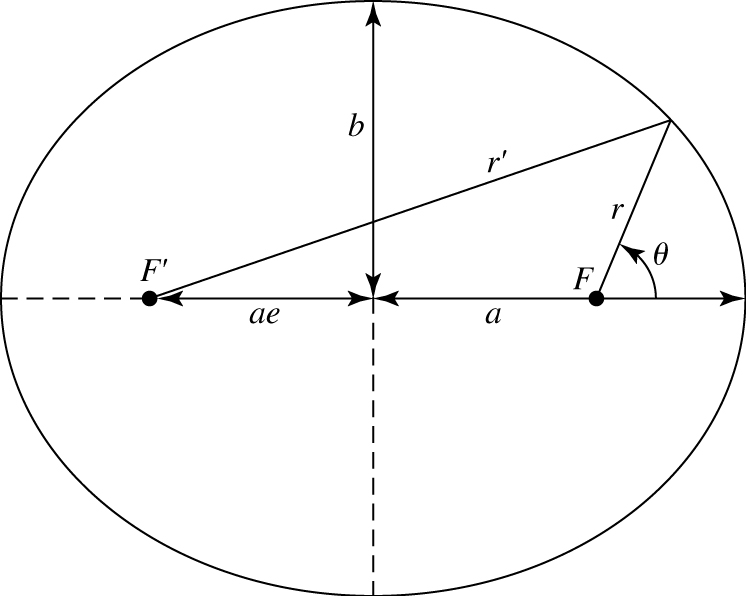
\includegraphics{planetarysystem.jpg}
		\caption{Geometry of an elliptical orbit. (Source:~Fig. 4, Chapter 2 of Carroll and Ostlie)}
		\label{carroll}
	\end{figure}
	\newpage
	We also define a few terms relevant to the physical system here:
	\begin{itemize}
		\setlength{\parskip}{0pt}
		\setlength{\itemsep}{0pt}
		\item \textbf{Perihelion}: The closest point to the Sun in the orbit.
		\item \textbf{Aphelion}: The farthest point to the Sun in the orbit.
		\item \textbf{Semi-major Axis}: Already defined, but in the version of Fig. \ref{carroll} without the guiding lines, it is equal to half the distance between the Perihelion and Aphelion. It is also the average distance of the Earth from the Sun. 
		\item \textbf{True Anomaly}: This is the angle $\theta$ in Fig. \ref{carroll}, which determines the position of the planet in the orbit. We will see two other anomalies (Eccentric and Mean) later.
		\item \textbf{Eccentricity}: Sounds familiar because it is. The eccentricity of the orbit can be found with the Perihelion and Aphelion distances. Definition is \href{http://staffhome.ecm.uwa.edu.au/~00043886/humour/invalid.proofs.html#1.2Proofbyintimidation}{trivial} and left as an exercise to the \href{http://staffhome.ecm.uwa.edu.au/~00043886/humour/invalid.proofs.html#1.6Proofbyomission}{reader}.
	\end{itemize}
	As there are other orbits apart from the Ellipse (Newton, 1687). These turn out to be the other conic sections. As \st{luck} math would have it, they are described by the same Equation~\ref{conic} that describes an ellipse.
	\begin{equation*}
		r = \frac{a(1-e^2)}{1 + e\cos \theta}
	\end{equation*}
	\begin{figure}[!h]
		\centering
		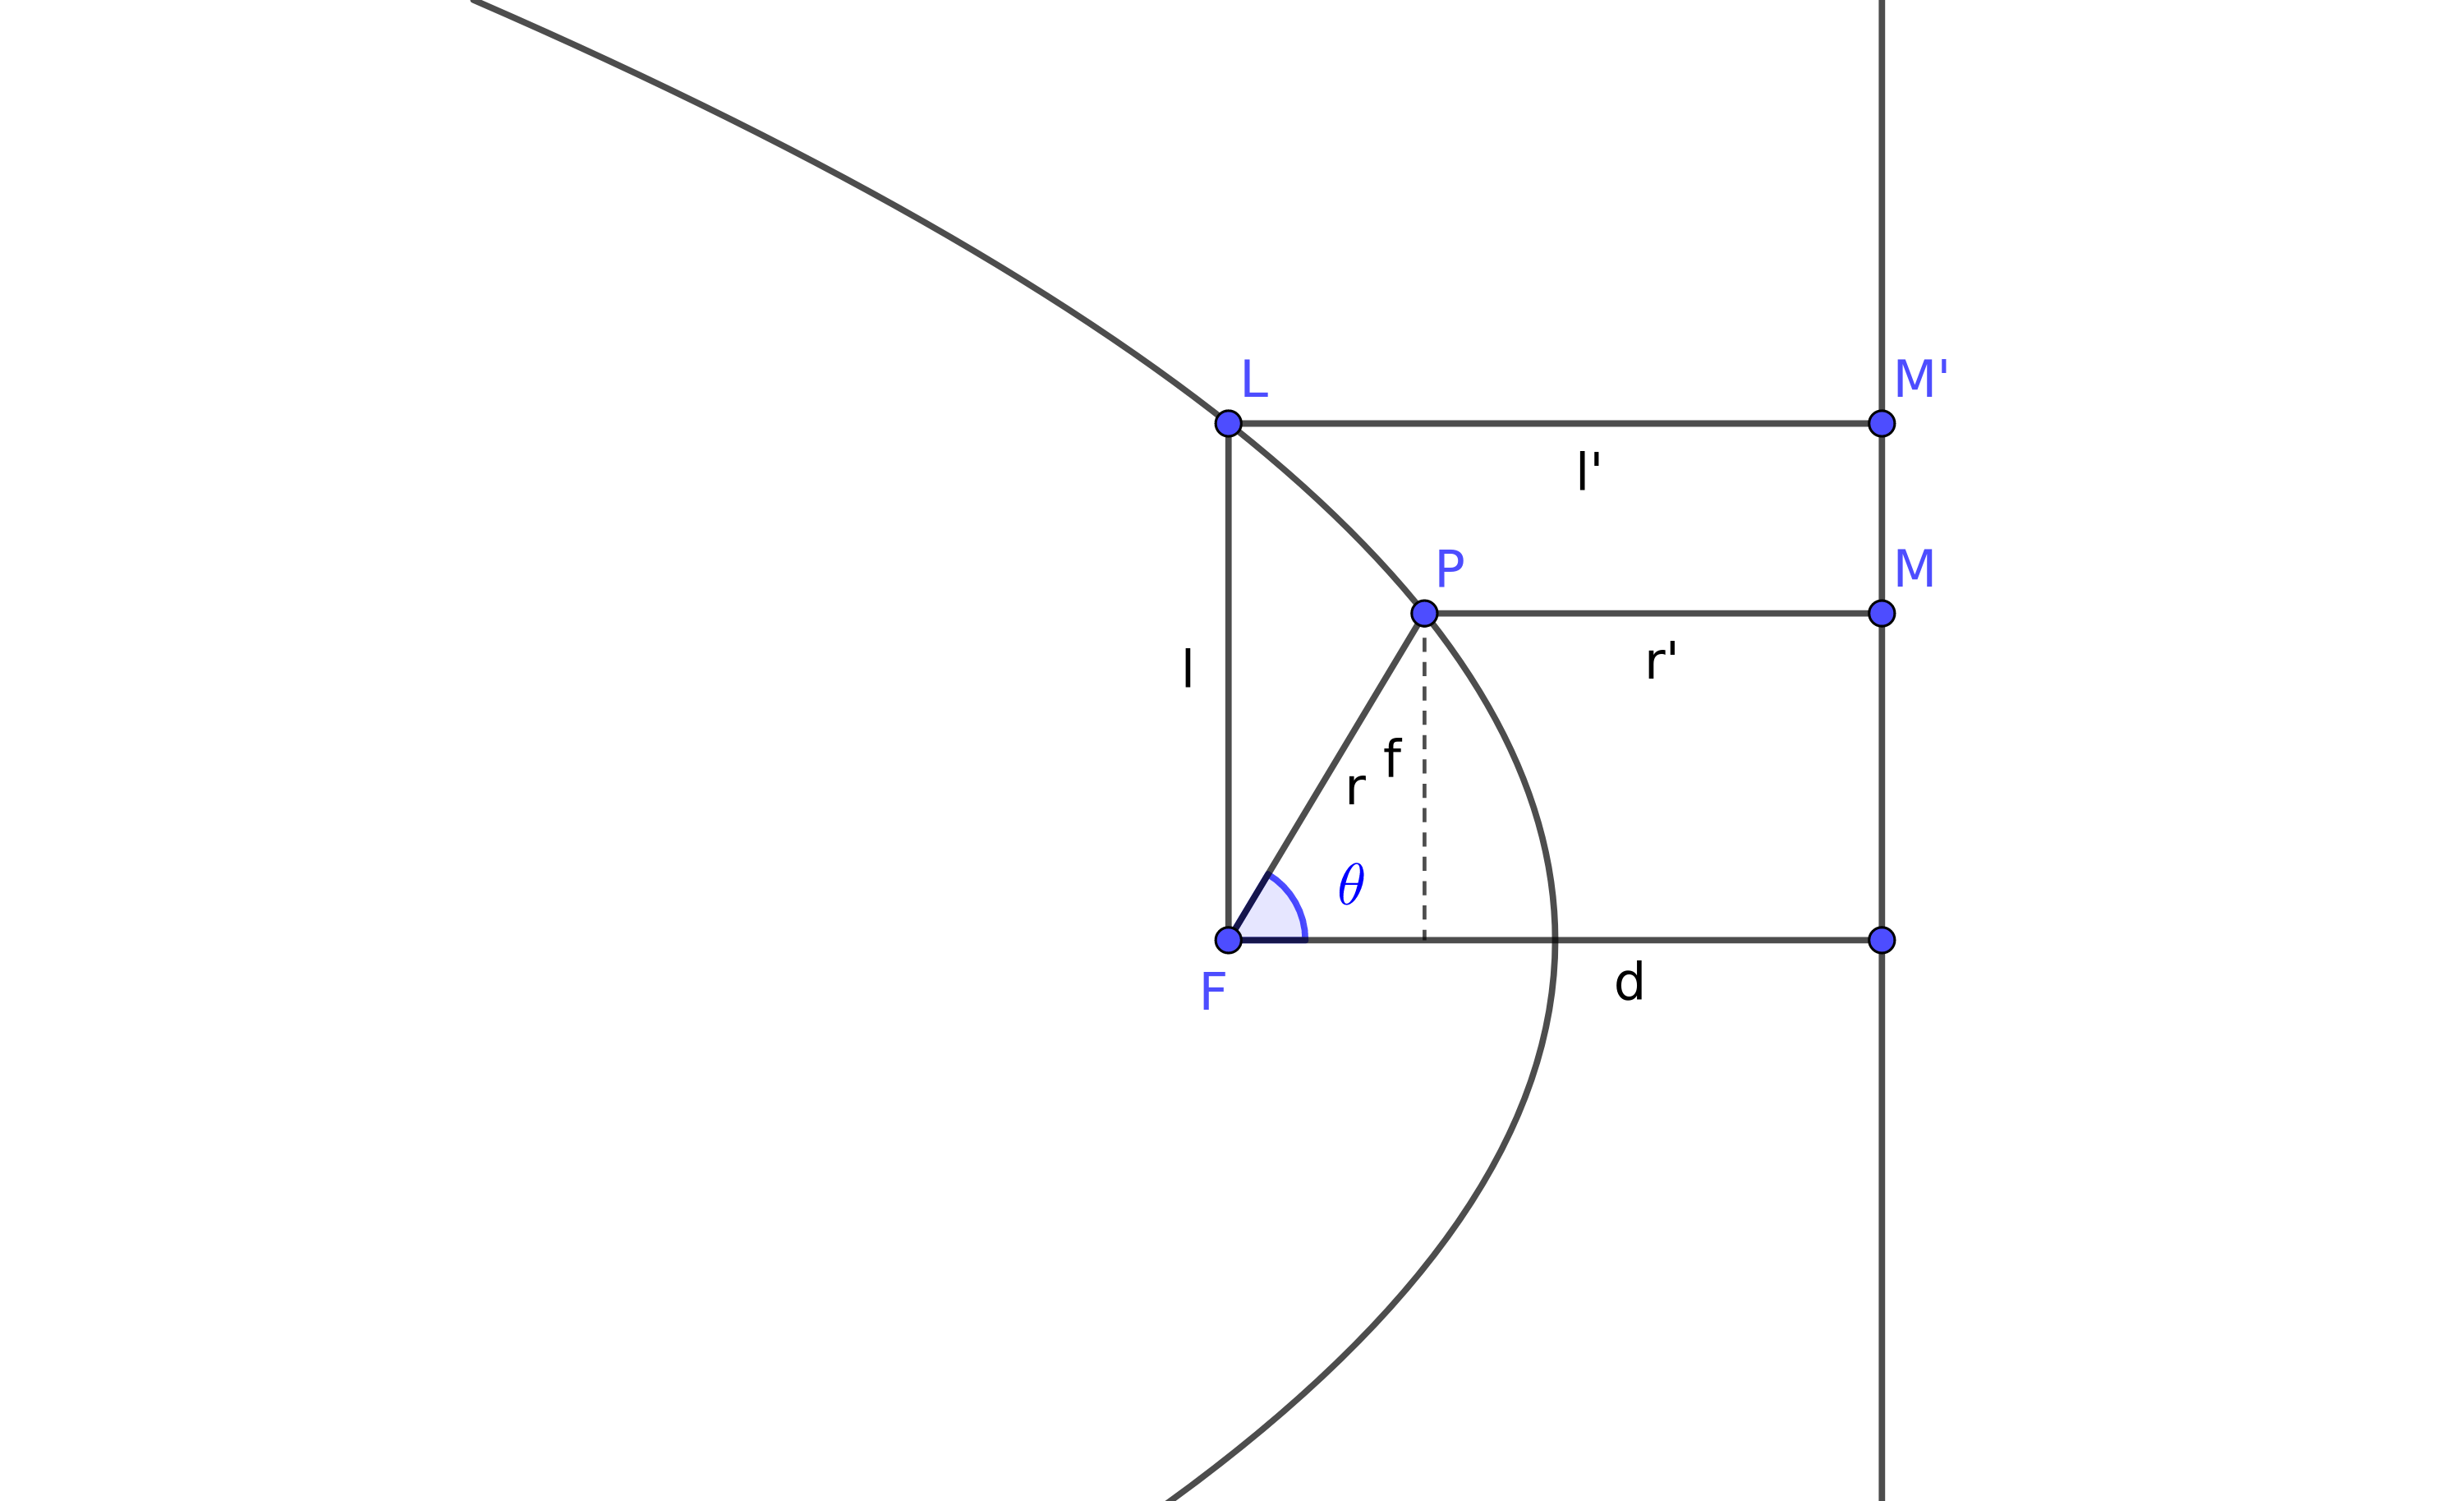
\includegraphics{conicderivation.png}
		\caption{Derive the equation of a conic section in polar coordinates (i.e. Eq. \ref{conic})}
		\label{conic_derivation}
	\end{figure}
\newline
	In Fig. \ref{conic_derivation}, we define the perpendicular distance from the Focus to the Directrix as $d$. another new quantity is the distance $l$, which we will call \emph{semi-latus rectum}, because that is what it is \href{http://staffhome.ecm.uwa.edu.au/~00043886/humour/invalid.proofs.html#15.5Proofbyparent}{called}. We have already seen this quantity in the numerator of Equation \ref{conic}. From Definition~2, we know that
	\begin{equation}
	\frac{r'}{r}=\frac{l'}{l}=\e
	\end{equation}
	Since it is \href{http://staffhome.ecm.uwa.edu.au/\~{}00043886/humour/invalid.proofs.html\#1.19Proofbypicture}{clear} that $l'=d$, and also that
	\begin{equation}
		r\cos\theta + r' = d
	\end{equation}
	Using these relations and some algebra, we will get
	\begin{equation}
		r = \frac{l}{1+e\cos\theta}
	\end{equation}
	And it is verifiable that for an ellipse, $l = a(1-e^2)$
\end{document}
